\documentclass[a4paper,oneside]{article}

\usepackage[linesnumbered,vlined,boxed]{algorithm2e}
\SetAlgorithmName{Behaviour}{behaviour}{List of Behaviours}

\usepackage{minitoc}
\setcounter{secttocdepth}{5}
\setcounter{tocdepth}{1}

\usepackage{graphicx}
\usepackage{epstopdf}
\usepackage[export]{adjustbox}
\usepackage[titletoc,title,header,page]{appendix}

\author{Philip Hale}
\title{CS3017 Assessment: A Power-Law Peer-to-Peer System}

\begin{document}

\begin{titlepage}
  \maketitle
  %\vfill
  \begin{abstract}
  A peer-to-peer system consisting of Super Peers and Ordinary Peers, operating
  in a power-law topology. The peers interact to exchange files using the
  document routing P2P model. The application is implemented in the Java Agent
  DEvelopment Framework (JADE), and ships with a default configuration that
  simulates `Scenario 1', where one peer has a file which all other peers want.
  See Appendix 1 For details on configuration and running the simulation.
  \end{abstract}
  \dosecttoc
  \tableofcontents
\end{titlepage}

\section{Peer Behaviour}

\secttoc

The system consists of three types of agent: Super Peers, Ordinary Peers and a
single Host Cache.  The Host Cache is implemented as an agent in order to unify
the connection behaviour between elements of the system.  In other words, peers
can connect to the Host Cache using the same mechanisms that are required to
connect to each other.

It can be helpful to think of the identity of an agent as defined by the kinds
of behaviours it can support. What we mean here by a behaviour is the ability to
respond in some way to a particular situation or event.  Some behaviours
continually monitor the state of the agent in the network, whereas others
are triggered by incoming messages from other agents.

The process of specifying and identifying different messages is explained in
another section.

Super Peers and Ordinary Peers implement a common set of behaviours. For
the sake of simplicity, the designation of peers into Super and Ordinary sets
will occur during initialization of the system.

In these examples, some simplifications have been made.  For example, we ignore
the difference between a file and hash of the file which identifies it. When an
algorithm states that it sends a file, it can be assumed that it is sending a
hash of the file.  In addition, this masks the fact that a peer will have a hash
table of some sort in order to identify the file from the file name.

Assumptions have been made that connections will not be lost, and that messages
will only be sent by peers that should send them.

In the following algorithms, the input for behaviours beginning with `Receive'
include a message name.  In effect this means ``the behaviour is triggered by a
message with this name''.

\subsection{Host Cache}

The Host Cache is the entry-point for the network with two responsibilities.
Firstly, to maintain a list of connected peers. Secondly, to supply peers with a
list of Super Peers which they can attempt to connect to

Theses behaviours can be summarised by the following piece of pseudocode. It
will run when the Host Cache receives a message identified as `Neighbours
Request'.

\subsubsection{Receive `Neighbours Request`}

\begin{algorithm}[H]
  \SetKwInOut{Input}{input}
  \SetKwFunction{SendFn}{send}
  \Input{Sender: $peer$ \\ Message Name: `Neighbours Request'}
  \KwData{$peerList$: A hash of peers with value true if peer is super}

  \If{peer list doesn't contain $peer$}{
    add $peer$ to $peerList$\;
  }
  \For{$connectedPeer \in peerList$}{
    \If{$peerList[connectedPeer] = true$ and $connectedPeer \neq peer$}{
      $neighbours \leftarrow neighbours \cup peer$\;
    }
  }
  \SendFn{peer, `Neighbours Response', neighbours}\;
\end{algorithm}

\subsection{All Peers}

Here we will explain the different types of behaviours implemented by both Super
and Ordinary Peers. Some of these behaviours are shared between all peers, but
their effects will differ depending on whether the peer is Super or Ordinary.
This is a design decision which compromises simplicity of the described
behaviours with simplicity of the system as a whole.\footnote{The idea is
analogous to the contradiction between two rules of software engineering: The
Law of Demeter which aims to minimise method chaining, and the idea of class
cohesion which gives an object well-bounded behaviour.}

\subsubsection{Send `Neighbours Request'}

The first message a peer will send: asks the Host Cache for a list of peers
which it can connect to in order to join the network. In addition, this message
is sent whenever the knownPeers list is empty.  This ensures that the peer
always has some Super Peer address to connect to, in the event that they need
more connections.

It only sends the request if the number of known peers is below a certain
maximum. Additionally, it only sends the request if it isn't already waiting for
a reply.

\begin{algorithm}[H]
  \SetKwFunction{SendFn}{send}
  \KwData{$knownPeers$: A list of neighbours known but not connected to the
  peer}
  \KwData{$hostCache$: Address of the Host Cache}
  \KwData{$hasRequestedPeers$: True if waiting for reply}
  \KwData{$isSuper$: True if the peer has sufficient bandwidth to be a Super
  Peer }

  \If{$knownPeers = \emptyset$ and $\neg hasRequestedPeers$}{
    \SendFn{hostCache, `Neighbours Request', isSuper}\;
    $hasRequestedPeer \leftarrow true$\;
  }
\end{algorithm}

\subsubsection{Receive `Neighbours Response'}

A reply to the `Neighbours Request' message. The message payload contains a
list of Super Peers which the peer can try and connect to.

\begin{algorithm}[H]
  \SetKwInOut{Input}{input}
  \Input{Message Name: `Neighbours Response' \\ Potential Neighbours: $peers$}
  \KwData{$hasRequestedPeers$: True if waiting for reply}
  \KwData{$knownPeers$: A list of Super Peers known but not connected to the
  peer}

  $knownPeers \leftarrow knownPeers \cup  peers$\;
  $hasRequestedPeer \leftarrow false$\;
\end{algorithm}

\subsubsection{Send `Connect Request'}

Asks a Super Peer to be a connection. In order to prevent blocking, the
contacted Super Peer is placed in a list while we wait for a response. 

The peer will keep trying to connect to more peers until the number of connected
peers is greater than a given minimum. In order to limit on how many connection
attempts are made, the count includes peers which we are waiting on for a reply.

\begin{algorithm}[H]
  \SetKwFunction{SendFn}{send}
  \KwData{$knownPeers$: A list of Super Peers known but not connected to the peer}
  \KwData{$connectPendingPeers$: Super Peers that have been sent a connection request}
  \KwData{$connectedPeers$: Super Peers that this peer is connected to}
  \KwData{$minPeers$: Required number of connected peers.}

  \If{$knownPeers \neq \emptyset $ {and} $\|connectPendingPeers \cup
  connectedPeers\| < minPeers$}{
    \SendFn{$ \exists p \in knownPeers$, `Connect Request'}\;
  }
\end{algorithm}

\subsubsection{Receive `Connect Response'}

A connection response is either successful or unsuccessful.  An alternative
approach would only send a response to the request if it is successful, but this
increases the complexity of the behaviour and so has not been adopted.

A connection response from a peer removes that peer from the known peers list.
If the connection is successful, the peer is also added to the list of connected
peers.

\begin{algorithm}[H]
  \SetKwInOut{Input}{input}
  \Input{Sender: $sender$ \\ Message Name: `Connect Response' \\ Connection
  Successful?: $connectSucceed$}
  \KwData{$knownPeers$: A list of Super Peers known but not connected to the peer}
  \KwData{$connectPendingPeers$: Super Peers that have been sent a connection request}
  \KwData{$connectedPeers$: Super Peers that this peer is connected to}

  $knownPeers \leftarrow knownPeers \setminus \{sender\}$\;
  $connectPendingPeers \leftarrow connectPendingPeers \setminus \{sender\}$\;
  \If{$connectSucceed = true$}{
    $connectedPeers \leftarrow connectedPeers \cup \{sender\}$\;
  }
\end{algorithm}

For this demonstration, a peer will always and continually search for files they
want.

\subsubsection{Send `Search Request'}

\begin{algorithm}[H]
  \SetKwFunction{SendFn}{send}
  \KwData{$connectedPeers$: Super Peers that this peer is connected to}
  \KwData{$wantedFiles$: List of files the peer wants but does not have}

  \If{$wantedFiles \neq \emptyset$ {and} $connectedPeers \neq \emptyset $}{
    \SendFn{$\exists p \in connectedPeers$, `Search Request', $\exists f \in
    wantedFiles$}\;
  }
\end{algorithm}

\subsubsection{Receive `File Request'}

Since our simulation does not send actual files, at this point we can simply
return a token response to indicate that we are transferring the file. In
practice, we would have to identify the file from the given identifier, and
check it exists before returning etc.

\begin{algorithm}[H]
  \SetKwInOut{Input}{input}
  \SetKwFunction{SendFn}{send}
  \Input{Sender: $peer$ \\ Message Name: `File Request' \\ File: $file$}
  \KwData{$sharedFiles$: List of files the peer wants but does not have}

  \SendFn{peer, `File Response', `Here is your file'}\;
\end{algorithm}

\subsubsection{Receive `File Response'}

This completes the procedure for acquiring files in the network.

\begin{algorithm}[H]
  \SetKwInOut{Input}{input}
  \SetKwFunction{SendFn}{send}
  \Input{Message Name: `File Response' \\ File: $file$ }
  \KwData{$sharedFiles$: List of files the peer wants but does not have}
  \KwData{$transferringFiles$: List of files that are waiting to be sent to this
  peer.}
  \KwData{$wantedFiles$: List of files the peer wants but doesn't have}

  \If{$file \in transferringFiles$}{
    $transferringFiles \leftarrow transferringFiles \setminus \{file\}$\;
    $wantedFiles \leftarrow wantedFiles \setminus \{file\}$\;
    $sharedFiles \leftarrow sharedFiles \cup \{file\}$\;
  }
\end{algorithm}

\subsection{Ordinary Peers}

These behaviours are exclusively implemented by Ordinary Peers.

\subsubsection{Send `File List'}

An Ordinary Peer is required to submit its list of shared files to its connected
Super Peer.  This is so that other peers can search for files.

Since this behaviour only applies to Ordinary Peers, we can make the simplifying
assumption that the list of connected peers only contains a single peer.

We also ignore the possibility that a SuperPeer can become disconnected, which
is not a requirement at this stage.

One further assumption is made.  We presume that the list of file hashes that
are sent to the Super Peer is small enough to fit in a single message. In
practice, this is not likely to be the case.

\begin{algorithm}[H]
  \SetKwFunction{SendFn}{send}
  \KwData{$connectedPeer$: Super Peer that this peer is connected to}
  \KwData{$sharedFiles$: List of files the peer wants but does not have}

  \SendFn{connectedPeer, `File List', sharedFiled}\;
\end{algorithm}

\subsubsection{Receive `Search Response'}

When a peer receives a search result, the nature of the protocol means that this
must be a successful result. If there is no results found, then there is simply
no message returned.  The payload of the message includes the particular file
that was found and the ID of the peer who owns it.  Since in our simulation we
do not need to present results in any way, once the result is found we can
contact the peer directly to request they transfer the file.

\begin{algorithm}[H]
  \SetKwInOut{Input}{input}
  \SetKwFunction{SendFn}{send}
  \Input{Message Name: `Search Response' \\ Result: $file$ \\ Peer With File:
  $peer$}
  \KwData{$transferringFiles$: List of files that have been requested
  from another peer, and are waiting to be sent to this peer.}
  \KwData{$wantedFiles$: List of files the peer wants but doesn't have}

  $wantedFiles \leftarrow wantedFiles \setminus \{file\}$\;
  \SendFn{peer, `File Request', file}\;
  $transferringFiles \leftarrow transferringFiles \cup \{file\}$\;
\end{algorithm}


\subsection{Super Peers}

These behaviours are exclusively implemented by Super Peers.

\subsubsection{Receive `Connection Request'}
input: a request from a peer to join; output: connection response (y/n)

Super Peers maintain a lit of peers which are connect to them, and the files
they are sharing.  The first step in this interaction is for the Peer to
associate itself with the Super Peer.

\begin{algorithm}[H]
  \SetKwFunction{SendFn}{send}
  \SetKwInOut{Input}{input}
  \Input{Sender: $peer$ \\ Message Name: `Connection Request'}
  \KwData{$connectedOrdinaryPeers$: Ordinary Peers that this peer is connected to}
  \KwData{$ordinaryPeerLimit$: Maximum number of Ordinary Peers this Super Peer
  can connect to}

  \eIf{$\|connectedOrdinaryPeers\| < ordinaryPeerLimit$}{
    $connectedOrdinaryPeers \leftarrow connectedOrdinaryPeers \cup \{peer\}$\;
    \SendFn{peer, `Connect Response', true}\;
  }{
    \SendFn{peer, `Connect Response', false}\;
  }
\end{algorithm}


\subsubsection{Receive `File list'}

The Super Peer stores the list of files for each Ordinary Peer it is connected
to. This is so that it is able to handle search requests.

The files are stored as a hash that maps $fileName \rightarrow peerList$.

\begin{algorithm}[H]
  \SetKwInOut{Input}{input}
  \Input{Sender: $peer$ \\ Message Name: `File List' \\ Shared Files:
  $fileList$}
  \KwData{$connectedOrdinaryPeers$: Ordinary Peers this peer is connected to}
  \KwData{$ordinaryPeersFiles$: All shared files of connected Ordinary Peers}

  \For{$file \in fileList$}{
    $ordinaryPeersFiles[file] \ peer$\;
  }
\end{algorithm}

\subsubsection{Receive `Search Response'}
%input: search response; output: nothing, or pass on search response

Super Peers must behave slightly differently when receiving a Search Response
message. Unlike for Ordinary Peers, sometimes this response may not be for them.
This is because search results do not get delivered directly: they are passed
back through intermediary peers using the Document Routing system.

It is worth noting that in our $send()$ function we pass as many arguments as we
have attributes. In practice, the attributes would be wrapped into a single
argument.

\begin{algorithm}[H]
  \SetKwInOut{Input}{input}
  \SetKwFunction{SendFn}{send}
  \Input{Message Name: `Search Response' \\ Result: $file$ \\ Peer With File:
  $peer$ \\ Previous Senders of the Search Response: $senderStack$}

  \uIf{$senderStack = \emptyset$}{
    inherit the behaviour of Ordinary Peer\;
  }{
    $superPeer \leftarrow senderStack.pop()$\;
    \SendFn{superPeer, 'Search Response', file, peer, senderStack}\;
  }
\end{algorithm}

\subsubsection{Receive `Search Request'}

%input: a file search request; output: either a search response, or a further
%search request (document routing).

When a Super Peer receives a Search Request for a file, it first checks its list
of files. If the file is found, it replies with a Search Response. 

If it is not found, it must pass on the message. If the $senderStack$ is empty
then the sender must be an ordinary peer, so the sender is added to it.  Next,
it adds itself to the $senderStack$ and passes on the message to $\exists peer
\in connectedOrdinaryPeers$.

The peer chosen to receive this message is picked based on the proximity of
their ID when compared to the file ID.  The details of this operation are not
explained in this section, but it introduces a requirement of the implemented
system for a consistent hashing algorithm.

\begin{algorithm}[H]
  \SetKwFunction{SendFn}{send}
  \SetKwFunction{NearestFn}{nearest}
  \SetKwInOut{Input}{input}
  \Input{Sender: $peer$ \\ Message Name: `Search Request' \\ Requested File:
  $file$ \\ Previous Senders of the Search Response: $senderStack$}
  \KwData{$connectedOrdinaryPeers$: Ordinary Peers connected to this Super Peer}
  \KwData{$ordinaryPeersFiles$: All shared files of connected Ordinary Peers}
  \KwData{$self$: This peer}

  \eIf{$ordinaryPeersFiles$ contains $file$}{
    $peerWithFile \leftarrow \exists p \in ordinaryPeersFiles[file] $\;
    \eIf{$senderStack = \emptyset$}{
      \SendFn{peer, `Search Response', file, peerWithFile}
    }{
      \SendFn{$senderStack.pop()$, `Search Response', file, peerWithFile,
      senderStack}\;
    }
  }{
    \tcc{We don't have the file; forward request to neighbour}
    $nearestNeighbour \leftarrow$ \NearestFn{senderStack, file}\;
    $senderStack \leftarrow senderStack \cup \{self\}$\;
    \SendFn{nearestNeighbour, `Search Request', file, senderStack}\;
  }

\end{algorithm}








\section{Protocols}

The following abbreviations are used:

\begin{description}
  \item[OPeer] An Ordinary Peer
  \item[SPeer] A Super Peer
  \item[Req.] Send a request message
\end{description}


\subsection{Joining the network}


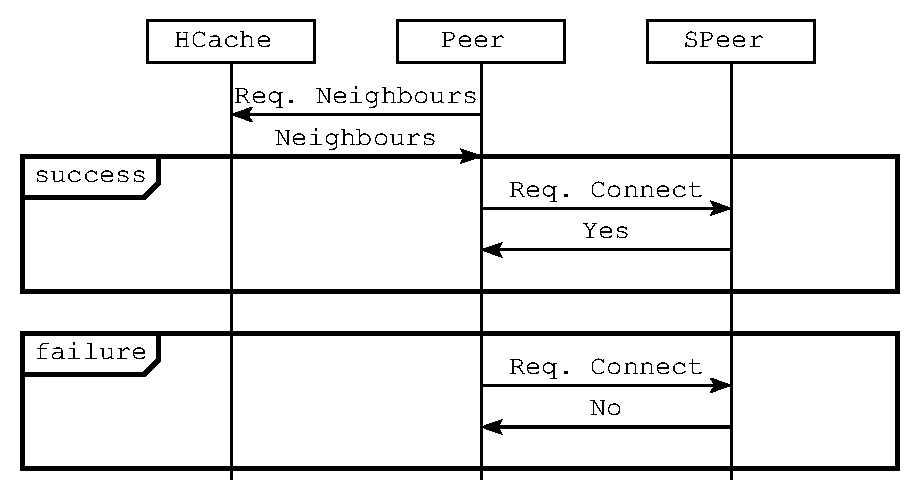
\includegraphics{protocol_connect.eps}



\section{Message Definitions}

\begin{itemize}
  \item{Neighbours Request}
  \item{Neighbours Response}
  \item{Search Request}
  \item{Search Response}
  \item{File Request}
  \item{File Response}
  \item{File List}
  \item{Connect Request}
  \item{Connect Response}
\end{itemize}




\begin{appendices}
  \section{Usage Instructions}
  mvn clean compile exec:java
\end{appendices}

\end{document}
